%%% Local Variables: 
%%% mode: pdflatex
%%% TeX-master: t
%%% End: 

\documentclass[onecolumn,x11names,technote,twoside,a4paper,10pt,english]{IEEEtran}
\usepackage[english]{babel}
\usepackage[pdftex]{graphicx}
\usepackage{amssymb}
\usepackage{amsmath}
\usepackage{caption}
\usepackage{float}
\usepackage{tikz}
\usepackage{euler}                                %Nicer numbers
\usepackage{listings}

\begin{document}

\title{Project in Digital Communication Systems}
\author{Noam~Lewis,~014740351  Zvulun~Avramov,~310877188}

\maketitle

\section{Answers to Preparatory Questions}

We have selected modulation number 5, entailing digital input data, $R_b=800$, QAM, and $B_{ch}=800Hz$. Because $R_s=\frac{R_b}{\log_2M}$, and the required bandwidth is $B_{min}=2R_s=800Hz$, we can calculate $M$:
\begin{eqnarray*}
  \log_2M &=& \frac{R_b}{R_s} \\
  &=& \frac{2R_b}{B_{min}} \\
  &=& \frac{1600}{800} = 2
\end{eqnarray*}
Therefore, $M=4$ so we are using 4QAM. Choosing symmetric symbols yields $A_n \in \{\pm \sqrt{1/2} \pm j \sqrt{1/2} \}$ with $|A_n|=1$ and $\phi_n \in \{ \pi/4, 3\pi/4, 5\pi/4, 7\pi/4 \}$. 

\begin{enumerate}
\item The modulated message $s_M(t)$ is:
  \begin{eqnarray*}
    \label{eq:s_M}
    s_M(t) &=& Re\{s_d(t)\sqrt{2P_c}e^{j\omega_c t}\} \\
           &=& \sqrt{2P_c}\sum_n{|A_n| g(t-n T_s) cos(\omega_ct + \phi_n)} \\
           &=& \sqrt{2P_c}\sum_n{ |A_n| cos(\phi_n) g(t-n T_s) cos(\omega_ct) - |A_n| sin(\phi_n) g(t-n T_s) sin(\omega_ct)} \\
           &=& \sqrt{2P_c}\sum_n{ A_{n_i} g(t-n T_s) cos(\omega_ct) - A_{n_q} g(t-n T_s) sin(\omega_ct)}
  \end{eqnarray*}
  Where  $A_n=A_{n_i}+jA_{n_q}=|A_n|e^{j\phi_n}=e^{j\phi_n}$.
  In the case of $t \in K T_s$, where $K \in \mathbb{Z}$, we can use the fact that $\forall t \notin n T_s : g(t-n T_s)=0$, and $1$ otherwise to arrive at:
  \begin{eqnarray*}
    s_M(t \in K T_s) &=& \sqrt{2P_c} cos(\omega_c t + \phi_K) \\
                     &=& \sqrt{2P_c} \left[ cos(\phi_K)cos(\omega_c t) - sin(\phi_K)sin(\omega_c t) \right] \\
                     &=& \sqrt{2P_c} \left[ A_{K_i}cos(\omega_c t) - A_{K_q}sin(\omega_c t) \right] 
  \end{eqnarray*}
\item Using known results from DSB modulation, and because we have a full response filter, and assuming that the symbols have expectation $0$:
  \begin{eqnarray*}
    S_M(f) &=& \frac{P_c}{2}(S_d(f-f_c)+S_d(f+f_c)) \\
    G(f)   &=& T_s sinc(\pi f T_s)e^{-j\pi f T_s} \\
    |G(f)|^2 &=& T_s^2 sinc^2(\pi f T_s)        \\
    S_d(f) &=& \frac{\sigma_a^2}{T_s} |G(f)|^2 =  T_s\sigma_a^2 sinc^2(\pi f T_s) \\
    \sigma_a^2 &=& \sum_{k=1}^M{p_k A_k^2} = \frac{1}{4} 4 = 1
  \end{eqnarray*}
  Substituting $S_d$ into $S_m$ we get:
  \begin{equation}
    \label{eq:S_M(f)}
    S_M(f) = \frac{P_c}{2R_s}\left[ sinc^2(\pi T_s(f-f_c)) + sinc^2(\pi T_s(f+f_c)) \right]
  \end{equation}
  The graph of $S_M(f)$ with example parameters is show in Figure \ref{fig:S_M(f)}.
  \begin{figure}[h!]
    \centering
    \input{q2.latex}
    \caption{$S_M(f)$ for $R_s=T_s^{-1}=10,f_c=100$}
    \label{fig:S_M(f)}
  \end{figure}
  When there is no noise in the channel, and with ideal synchronization the demodulated signal is:
    \begin{eqnarray*}
      x_{d_i}(t) &=& x(t)A_0 cos(\omega_c t) \\
                &=& A_0\sqrt{2P_r} cos(\omega_c t + \phi_K) cos(\omega_c t) \\
                &=& A_0\sqrt{\frac{P_r}{2}} \left[ cos(\phi_k) + cos(2\omega_c t + \phi) \right] \\
      x_{d_q}(t) &=& -x(t)A_0 sin(\omega_c t) \\
                &=& A_0\sqrt{\frac{P_r}{2}} \left[ sin(\phi_k) + sin(2\omega_c t + \phi) \right] 
    \end{eqnarray*}
  If $x_{d_i}(t)$ for example passes through the appropriate matched filter, the output is:
  \begin{eqnarray*}
    a_{k_i} &=& \int_{kT_s}^{(k+1)T_s}{ x_{d_i}(t) g(t-kT_s) dt} \\
           &=&  \int_{kT_s}^{(k+1)T_s}{ A_0\sqrt{\frac{P_r}{2}} \left[ cos(\phi_k) + cos(2\omega_c t + \phi) \right]  dt} \\
           &=&  A_0\sqrt{\frac{P_r}{2}} T_s cos(\phi_k) + \int_{kT_s}^{(k+1)T_s}{ cos(2\omega_c t + \phi)  dt} 
  \end{eqnarray*}
  If $R_s \to m (2f_c)$ where $m \in \mathbb{N}$, the integral goes to zero, and we are left with:
  \begin{eqnarray*}
    a_{k_i} &=& A_0\sqrt{\frac{P_r}{2}} T_s cos(\phi_k) = \frac{\sqrt{P_r} A_{k_i}}{R_s} \\
    a_{k_q} &=& A_0\sqrt{\frac{P_r}{2}} T_s sin(\phi_k) = \frac{\sqrt{P_r} A_{k_q}}{R_s}
  \end{eqnarray*}
  Where the right hand sides result from choosing $A_0=\sqrt{2}$. Combining the components gives:
  \begin{equation}
    \label{eq:a_k}
    a_k = a_{k_i} + j a_{k_q} = \frac{\sqrt{P_r}}{R_s} A_k
  \end{equation}

\item For a symbol dictionary of size $M$: $R_s=\frac{R_b}{\log_2M}$ and $K_b=\log_2M$.

\item In Gray coding, every two consequetive numbers differ by exactly one bit. The encoding reduces BER by assigning similar codes to closer symbols. The probability of receiving a symbol in close vicinity to the transmitted one is higher, so errors with small number of bit flips are more probable. In our case (where $M=4$) we can assign:

  \begin{center}
    \begin{table}[h!]
      \centering
      \begin{tabular}[h!]{| l | l | l |}
      \hline
      Code & Symbol & \\ \hline
      $00$ & $+\sqrt{1/2}+j\sqrt{1/2}$ & $A_1$  \\ \hline
      $01$ & $-\sqrt{1/2}+j\sqrt{1/2}$ & $A_2$  \\ \hline
      $11$ & $-\sqrt{1/2}-j\sqrt{1/2}$ & $A_3$  \\ \hline
      $10$ & $+\sqrt{1/2}-j\sqrt{1/2}$ & $A_4$  \\
      \hline
      \end{tabular}
      \caption{Assignment of bit patterns to symbols}
      \label{tab:bitsymbols}
    \end{table}
  \end{center}

\item The symbol constellation is shown in Figure \ref{fig:4qam-const}. 
  \begin{figure}[h!]
    \begin{center}
      \begin{tikzpicture}[scale=3]
        % Circles 
        \foreach \r in { 1}
        \draw[Azure4, thin] (0,0) circle (\r);
        % 45� Rays
        \foreach \a in {0, 45,...,359}
        \draw[Azure4] (\a:1) -- (\a:1.5);
        % Radius labels (background filled white)
        \draw (0.707,0) node[inner sep=1pt,below=3pt,rectangle,fill=white] {$\frac{1}{\sqrt{2}}$};
        \draw (0,0.707) node[inner sep=1pt,left=3pt,rectangle,fill=white] {$j\frac{1}{\sqrt{2}}$};
        \draw (-0.707,0) node[inner sep=1pt,below=3pt,rectangle,fill=white] {$-\frac{1}{\sqrt{2}}$};
        \draw (0,-0.707) node[inner sep=1pt,left=3pt,rectangle,fill=white] {$-j\frac{1}{\sqrt{2}}$};
        % Main rays
        \foreach \a in {0, 90,...,359}
        \draw[very thick] (0, 0) -- (\a:1.5);
        % Angle labels  
        \foreach \a in {0, 45,...,359}
        \draw (\a: 1.6) node {$\a^\circ$};
        % Central point
        \draw[fill=red] (0.707,0.707) circle(0.4mm) node[inner sep=1pt,below=4pt,rectangle] {$00$};
        \draw[fill=red] (-0.707,0.707) circle(0.4mm)  node[inner sep=1pt,below=4pt,rectangle] {$01$};
        \draw[fill=red] (-0.707,-0.707) circle(0.4mm)  node[inner sep=1pt,below=4pt,rectangle] {$11$};
        \draw[fill=red] (0.707,-0.707) circle(0.4mm)  node[inner sep=1pt,below=4pt,rectangle] {$10$};
      \end{tikzpicture}
    \end{center}
    \caption{Constellation of symbols. Each node is labeled with the assigned (gray coded) bit pattern.}
    \label{fig:4qam-const}
  \end{figure}

\item The Euclidean distance between adjacent symbols is $\frac{2}{\sqrt{2}}=\sqrt{2}$. In terms of phase drift, the distance is $\pi/4$.

\item Effects of channel on the communication system:
  \begin{enumerate}
  \item AWGN - The noise appears as an additive element in the symbols entering the decision device. If $a_k$ is the portion originating from the source signal, and $z_k$ is the effect of the noise, then $q_k = a_k + z_k$. For a time period where $t \in k T_s$ we have:
    \begin{eqnarray*}
      x(t) &=& s_r(t) + n_r(t) \\
      s_r(t) &=& k_{ch}s_M(t) = \sqrt{2P_r} \left[ cos(\phi_K)cos(\omega_c t) - sin(\phi_K)sin(\omega_c t) \right]  \\
      n_r(t) &=& n_{r_i}(t)cos(\omega_c t) - n_{r_q}(t) sin(\omega_c t) \\
    \end{eqnarray*}
    The noise component affects $\text{SNR}_d$. The relevant parameter is the noise power (variance) $\sigma_z^2$.

  \item Limited channel bandwidth - ISI (Inter Symbol Intereference): In this case the received symbol $q_k$ has an additional component, the ISI: $q_k = p_0A_K + \sum_{n \neq k} {A_n p_{k-n}} + z_k$. This effect can be countered by, for example, an optimal sequential detector.

  \item Phase and Frequency shift - after demodulation (separately for the two bases), we get:
    \begin{eqnarray*}
      x_{d_i}(t) &=& x(t)A_c cos(\omega_c t) \\
                &=& A_c\sqrt{2P_r} cos(\omega_r t + \phi_K + \Psi) cos(\omega_c t) + A_c cos(\omega_c t) n_r(t)\\
                &=& A_c\sqrt{\frac{P_r}{2}} cos(\phi_k + \Psi + \Delta \omega t) 
                    + \underbrace{ \frac{A_c}{2} \left( n_{r_i}(t) + n_{r_q}(t) \right) }_{\mbox{additive noise component}} 
                    + \text{ Higher frequency components} \\
      x_{d_q}(t) &=& -x(t)A_c sin(\omega_c t) = A_c\sqrt{\frac{P_r}{2}} sin(\phi_k + \Delta \omega t + \Psi) + \text{ ... }
    \end{eqnarray*}
    Where $\Delta \omega = \omega_r - \omega_c$ is the frequency shift, and $\Psi$ is the phase shift. Since we are using 4-QAM, if the phase shift nears $\pi/8$ the symbols may be confused, so a phase synchronizer is required.
    
  \end{enumerate}

  \item Definitions of $\text{SNR}_{bit}^{(DD)}$ and $\text{SNR}_{sym}^{(DD)}$: 
    \begin{eqnarray*}
      \text{SNR}_{sym}^{(DD)} &=& \frac{P_{sym}}{P_{n_r}} = \frac{R_s E_s}{R_s N_0} = \frac{E_s}{N_0} \\
                            &=& \frac{P_rE_g}{N_0}\sum_{k=0}^{M-1}{p_k|A_k|^2 } \\
      \text{SNR}_{bit}^{(DD)} &=& \frac{\text{SNR}_{sym}^{(DD)}}{\log_2(M)}
    \end{eqnarray*}
    In our case, $\forall k:|A_k|^2=1$, $E_g=T_s=1/R_s$, and $\log_2(M)=2$, and we assume uniform symbol distribution ($p_k=1/M$) so:
    \begin{eqnarray*}
      \text{SNR}_{sym}^{(DD)} &=& \frac{P_r}{R_sN_0}\\
      \text{SNR}_{bit}^{(DD)} &=& \frac{P_r}{2R_sN_0}
    \end{eqnarray*}


\item $erfc(\lambda) = 2Q( \sqrt{2}\lambda )$, and $\frac{1}{2} erfc( \frac{\lambda}{\sqrt{2}} ) = Q(\lambda )$.

\item Because we are using code gray, the following relation holds whenever the SNR is high enough to make transitions to far symbols unlikely:
    \begin{equation*}
      P_{err,bit}^{(DD)} \approx \frac{P_{err,sym}^{(DD)}}{\log_2{M}} = \frac{P_{err,sym}^{(DD)}}{2}
    \end{equation*}
    The probability for symbol error is defined by:
    \begin{equation*}
      P_{err,sym}^{(DD)} = \sum_{m=1}^M {p_m P(\text{error} | A_m)} = \sum_{m=1}^M {p_m \left[ 1 - \prod_{n=1,n \neq m}^M \left( 1 - P(A_n | A_m) \right) \right]} 
    \end{equation*}
    Where, if $d_{m,n}= |A_m - A_n|$ is the Euclidean distance between symbols $A_m$ and $A_n$:
    \begin{equation*}
      P(A_n | A_m) = Q\left( \frac{d_{m,n}}{2 \sigma_z}\right)
    \end{equation*}
    In our case, $d_{m,n} = \sqrt{2}$ for neighboring symbols, and $d_{m,n} = 2$ for the non-neighboring ones. Due to the nature of the $Q$ function we can safely discard the terms for the probabilities between non-neighboring symbols.

    We want the probability expressed as a function of $\gamma_d$:
    \begin{equation*}
      \gamma_d = \frac{E_r}{N_0} 
    \end{equation*}
    We can calculate $E_r$ as follows:
    \begin{eqnarray*}
      E_r &=& \int_0^{T_s}{s^2_r(t) dt} \\
          &=& 2P_r \int_0^{T_s}{ \left[ A_{K_i}cos(\omega_c t) - A_{K_q}sin(\omega_c t) \right]^2 dt} \\
          &=& 2P_r \int_0^{T_s}{ \left[ A_{K_i}^2cos^2(\omega_c t) + A_{K_q}^2sin^2(\omega_c t) - \frac{1}{2} A_{K_i} A_{K_q} sin(2\omega_c t) \right] dt} \\
          && \{\text{Discarding higher-frequency components which would be filtered in the integration}\} \\
          &=& P_r \int_0^{T_s}{ \left[ A_{K_i}^2 + A_{K_q}^2 \right] dt} \\
          &=& \frac{P_r |A_{K}|^2}{R_s} = \frac{P_r}{R_s}
    \end{eqnarray*}
    Therefore,
    \begin{equation*}
      \gamma_d = \frac{P_r}{R_s N_0}
    \end{equation*}
    Using Equation \ref{eq:a_k} from question 2, we can express the distance between nearby symbols as:
    \begin{equation*}
      d_{m,n} = | \frac{\sqrt{P_r}}{R_s} (A_m - A_n) | = \frac{\sqrt{P_r}}{R_s} |A_m - A_n|
    \end{equation*}
    In our case for neighboring symbols $|A_m - A_n|=\sqrt{2}$ so:
    \begin{equation*}
      d_{m,n} = \frac{\sqrt{2P_r}}{R_s}
    \end{equation*}
    To find $\sigma_z$ we calculate the noise component output from the matched filter:
    \begin{eqnarray*}
      z_k &=& \int_{kT_s}^{(k+1)T_s}{ n_r(t) A_0 cos(\omega_c t) g(t-kT_s) dt} \\
          && \{\text{Discarding higher-frequency components}\} \\
          &=& \frac{A_0}{2} \int_{kT_s}^{(k+1)T_s}{ n_{r_i}(t) dt} 
    \end{eqnarray*}
    Assuming Gaussian white noise, because the integral (the matched filter) is a linear system we can calculate the variance (the power) as:
    \begin{eqnarray*} 
      \sigma_z^2 = \sigma_{n_r}^2 = \sigma_{n_{r_i}}^2 &=& \frac{1}{2}\int_{-\infty}^{\infty}{ S_{n_i}(f) |H_{MF}(f)|^2 df} \\
                 && \{\text{$n_{r_i}$ is baseband noise limited to $f \in R_s$ } \\
                 && \text{$H_{MF}$ is fourier transform of $g(t)$, rectangular pulse } \\
                 && \text{$\Rightarrow$ almost all energy of $H_{MF}$ is limited to $f \in R_s$}\} \\
                 &\approx& \frac{1}{2} \int_{-\infty}^{\infty}{ N_0  |H_{MF}(f)|^2 df} \\
                 &=& \frac{N_0}{2} \int_{-\infty}^{\infty}{  |H_{MF}(f)|^2 df} \\
                 && \{\text{Parseval's theorem}\} \\
                 &=& \frac{N_0}{2} E_g = \frac{N_0}{2R_s} 
    \end{eqnarray*}

    Thus,
    \begin{equation*}
      \frac{d_{m,n}}{2\sigma_z} = \frac{\sqrt{2P_r}}{R_s} \frac{1}{2 \sqrt{\frac{N_0}{2R_s}} }  = \frac{\sqrt{P_rR_s}}{R_s\sqrt{N_0 }} = \sqrt{\frac{P_r}{R_s N_0 }} = \sqrt{\gamma_d}
    \end{equation*}
    Finally,
    \begin{eqnarray*}
      P(A_n | A_m) &=& Q\left( \sqrt{\gamma_d}\right) \nonumber \\
      P_{err,sym}^{(DD)} &=& \sum_{m=1}^4 {p_m \left[ 1 - \prod_{n=1,n \neq m}^4 \left( 1 - Q\left( \sqrt{\gamma_d}\right) \right) \right]}
    \end{eqnarray*}
    Discarding higher-order Q's (including the ones for the non-neighboring symbols), and also assuming uniform symbol distribution ($p_m=1/4$), we arrive at:
    \begin{equation}
      \label{eq:P_errsym}
      P_{err,sym}^{(DD)} = 2Q\left( \sqrt{\gamma_d}\right) = \mathrm{erfc}(\sqrt{\gamma_d / 2})
    \end{equation}
    Inverting the expression, we get:
    \begin{equation}
      \label{eq:invP_errsym}
      \gamma_d = 2 \left({\mathrm{erfc}^{-1}}(P_{err,sym}^{(DD)}) \right)^2
    \end{equation}
    Thus, in Matlab, given symbol error probability $p$, we can calculate $\gamma_d$ as follows:
    \lstset{language=matlab}
    \lstset{keywordstyle=\bfseries}
    \lstset{morekeywords={erfcinv}}
    \begin{lstlisting}[label=lst:matlab_perr]{}
      gamma_d = 2*(erfcinv(p))^2
    \end{lstlisting}
    For convenience we also find the relation between the received noise variance and $\gamma_d$:
    \begin{equation} 
      \label{eq:sigma_noise_gamma}
      \sigma_{n_r}^2 = \frac{1}{2} N_0 2R_s = N_0 R_s = \frac{P_r}{\gamma_d}
    \end{equation}
    

\end{enumerate}

\clearpage
\section{Simulation}

\subsection{Data sets}
\begin{enumerate}
\item Small data set - the bit sequence: $\{0,0,1,1,1,0,0,1\}$, which corresponds to the sequence $\{A_1, A_3, A_4, A_2\}$.
\item Large (random) data set - a random stream of $5^3 \log_2M = 10^3$ bits. The data set was created by applying the function $f(x) = \text{\bf{ if }} x>0.5 \text{\bf{ then }} 1 \text{\bf{ else }} 0$ to each element of a vector constructed with the Matlab 'rand' function.
\end{enumerate}

\subsection{Transmitter}
The chosen sampling frequency was $8 f_c$, so that:
\begin{itemize}
\item Nyquist's criterion is met ($2 f_c$ would suffice)
\item Enough samples are shown in the Matlab graphs, to make the real amplitude visible.
\end{itemize}

The symbol/bit patterns appear in Table \ref{tab:bitsymbols}. The symbol constellation is shown in Figure \ref{fig:trans_constellation}.

\begin{enumerate}
\item $P_c = 10W$, therefore $A_c = \sqrt{20}$.
\item $f_c = 20kHz$ so $w_c = 4\pi \cdot 10^4$.
\item Sampling frequency (for simulation of the continuous signal) is $f_s = 2f_c = 40khz$.
\end{enumerate}

  \begin{figure}[h!]
    \centering
    \includegraphics[height=3.5in]{symbol_constellation.png}
    \caption{Constellation of symbols received}
    \label{fig:trans_constellation}
  \end{figure}

The time response of the small dataset is shown in Figure \ref{fig:s_M(t)}. The frequency response of the large (random) data set is show in Figure \ref{fig:S_M(f)}.

  \begin{figure}[h!]
    \centering
    \includegraphics[height=3.5in]{modulated_small_dataset.png}
    \caption{$s_M(t)$ for small data set}
    \label{fig:s_M(t)}
  \end{figure}

  \begin{figure}[h!]
    \centering
    \includegraphics[height=3.5in]{modulated_random_dataset_fft.png}
    \caption{$S_M(f)$ for large (random) data set}
    \label{fig:S_M(f)}
  \end{figure}

\subsection{Receiver, no noise}
\begin{enumerate}
\item Time domain graphs of signals: outputs of transmit filters in Figure \ref{fig:s_d(t)}; outputs of matched filters in receiver in Figure \ref{fig:q(t)}. The transmit filter simply outputs a constant function of the symbol because we use a full-response pulse ($g(t) = 1\ \forall t \in Ts\ ,\ 0\ \text{otherwise}$). The matched filter produces an integral of the demodulated signal re-starting from 0 at every symbol interval. We can see that the peak of the integral corresponds to the end of the symbol interval, and is equal to the value of the symbol that was transmitted.
  \begin{figure}[h!]
    \centering
    \includegraphics[height=3.5in]{transmit_filter_output.png}
    \caption{$s_{d_i}(t)$ and $s_{d_q}(t)$, outputs of the transmit filter (before modulation)}
    \label{fig:s_d(t)}
  \end{figure}
  \begin{figure}[h!]
    \centering
    \includegraphics[height=3.5in]{matched_filter_output.png}
    \caption{$q_i(t)$ and $q_q(t)$, sampled outputs of the matched filters (before decision device)}
    \label{fig:q(t)}
  \end{figure}

\item Symbols: for constant phase - ideal synchronization between transmitter and receiver. Table \ref{tab:recvsymbols} shows the values of the symbols received from the matched filter (after sampling). Figure \ref{fig:recv_constellation} shows the received symbols as a constellation. A comparison of the transmitted symbols with the received ones shows that they are quite close, as can be seen in Figure \ref{fig:zoom_constellation}. The errors (difference) between distances of transmitted symbols to those received are shown in Table \ref{tab:dist_recvsymbols}. The errors are small, and are due to the inprecise integration method ('trapz' Matlab function, trapezoid integration) used in the simulation. In an ideal system there would be no error in this case. Mathematically, the distances are 0.
  \begin{center}
    \begin{table}[h!]
      \centering
      \begin{tabular}[h!]{| l | l |}
      \hline
      k             &  Received Symbol  \\ \hline
      1             &  0.7035 + 0.7053j \\ \hline
      2             & -0.7035 - 0.7053j \\ \hline
      3             &  0.7053 - 0.7071j \\ \hline
      4             & -0.7053 + 0.7071j \\
      \hline
      \end{tabular}
      \caption{Symbols received (sampled matched filter output)}
      \label{tab:recvsymbols}
    \end{table}
  \end{center}
  \begin{figure}[h!]
    \centering
    \includegraphics[height=3.5in]{recv_symbol_constellation.png}
    \caption{Constellation of symbols received}
    \label{fig:recv_constellation}
  \end{figure}
  \begin{center}
    \begin{table}[h!]
      \centering
      \begin{tabular}[h!]{| l | l |}
      \hline
      Symbol    &  Distance \\ \hline
      $A_{r_1}$  &     0.0040 \\ \hline
      $A_{r_2}$  &     0.0018 \\ \hline
      $A_{r_3}$  &     0.0040 \\ \hline
      $A_{r_4}$  &     0.0018 \\ 
      \hline
      \end{tabular}
      \caption{Distances between symbols transmitted and those received}
      \label{tab:dist_recvsymbols}
    \end{table}
  \end{center}
  \begin{figure}[h!]
    \centering
    \includegraphics[height=3.5in]{trans_recv_symbol_constellation.png}
    \caption{Zoom on the first symbol $A_1$ - showing the transmitted and received symbols. \newline The dotted line represents a portion of the unit circle.}
    \label{fig:zoom_constellation}
  \end{figure}



\item Symbols: unsychronized phase channel - difference of $30^o$ between transmitted and received. Table \ref{tab:recvsymbols_phase} shows the values of the symbols received from the matched filter (after sampling). Figure \ref{fig:recv_constellation_phase} shows the received symbols as a constellation. A comparison of the transmitted symbols with the received ones shows that they are quite close, as can be seen in Figure \ref{fig:trans_recv_constellation_phase}. The distances between transmitted symbols to those received are shown in Table \ref{tab:dist_recvsymbols_phase}. The large errors are due to the phase difference between transmitter and receiver.
  \begin{center}
    \begin{table}[h!]
      \centering
      \begin{tabular}[h!]{| l | l |}
      \hline
      k             &  Received Symbol  \\ \hline
      1             &  0.7035 + 0.7053j \\ \hline
      2             & -0.7035 - 0.7053j \\ \hline
      3             &  0.7053 - 0.7071j \\ \hline
      4             & -0.7053 + 0.7071j \\
      \hline
      \end{tabular}
      \caption{Symbols received with phase difference of $pi/6$ (sampled matched filter output)}
      \label{tab:recvsymbols_phase}
    \end{table}
  \end{center}
  \begin{figure}[h!]
    \centering
    \includegraphics[height=3.5in]{recv_symbol_constellation_phase.png}
    \caption{Constellation of symbols received with phase difference of $pi/6$}
    \label{fig:recv_constellation_phase}
  \end{figure}
  \begin{center}
    \begin{table}[h!]
      \centering
      \begin{tabular}[h!]{| l | l |}
      \hline
      Symbol    &  Distance \\ \hline
      $A_{r_1}$  &  0.5155   \\ \hline
      $A_{r_2}$  &  0.5185   \\ \hline
      $A_{r_3}$  &  0.5155   \\ \hline
      $A_{r_4}$  &  0.5185   \\ 
      \hline
      \end{tabular}
      \caption{Distances between symbols transmitted and those received with phase difference of $pi/6$}
      \label{tab:dist_recvsymbols_phase}
    \end{table}
  \end{center}
  \begin{figure}[h!]
    \centering
    \includegraphics[height=3.5in]{trans_recv_symbol_constellation_phase.png}
    \caption{Constellation of the transmitted and received symbols with phase difference of $pi/6$. \newline The dotted line represents the unit circle.}
    \label{fig:trans_recv_constellation_phase}
  \end{figure}
\end{enumerate}

\clearpage
\subsection{Receiver, with noise}
Using Matlab and the definition in Equation \ref{eq:invP_errsym}, we calculate: 
\begin{itemize}
\item $p_{err}=10^{-3} \Rightarrow \gamma_{d_{max}} = 10.8276 = 3.3339 \mathrm{[dB]} $
\item $p_{err}=0.2 \Rightarrow \gamma_{d_{min}} = 1.6424 = 10.1474 \mathrm{[dB]}$
\end{itemize}
The following simulation was repeated for the following set of SNR values: $\gamma_d \in {2.1547,\ 4.1547,\ 6.1547,\ 8.1547,\ 10.1547}$. To produce bandlimited gaussian white noise in Matlab, we:
\begin{enumerate}
\item create a vector of random samples using normal distribution, n(t), 
\item filter the random vector using Matlab's 'fir1' and 'filter' functions with appropriate bandwidth.
\end{enumerate}
Before filtering, the random samples have power density in the range of the sampling frequency. We have a target variance (given by Equation \ref{eq:sigma_noise_gamma}). Thus, to calculate the proper variance to use in the creation of the vector, we use our sampling frequency of $f_s = 8f_c$:
\begin{equation*}
  \sigma_{n_{sim}}^2 = \frac{f_s N_0}{2} = \frac{4 P_r f_c}{R_s \gamma_d}
\end{equation*}
This way, after filtering we will have the appropriate variance (power). Because the filtering is only an approximation of an ideal rectangular filter, we have decided to use the basic 'fir1' Matlab filter and choose an order parameter that gives (approximately) the same power density in the bandwidth region as before filtering. The order we found was 70.

We have simulated an AWGN channel, using a 5,000 bit random transmission. After receiving, the number of incorrect bits was counted and normalized to calculate the bit error rate. Figure \ref{fig:BER_noise} presents the result of the simulation as opposed to the analytical calculation of the probability of bit error, when the phase is ideally synchronized (zero phase difference). Figure \ref{fig:BER_noise_phase} shows the results for two constant phase differences. The resulting graphs are averaged over 10 repetitions with different random noises. Both graphs include error bars indicating the standard deviation of the results.
  \begin{figure}[h!]
    \centering
    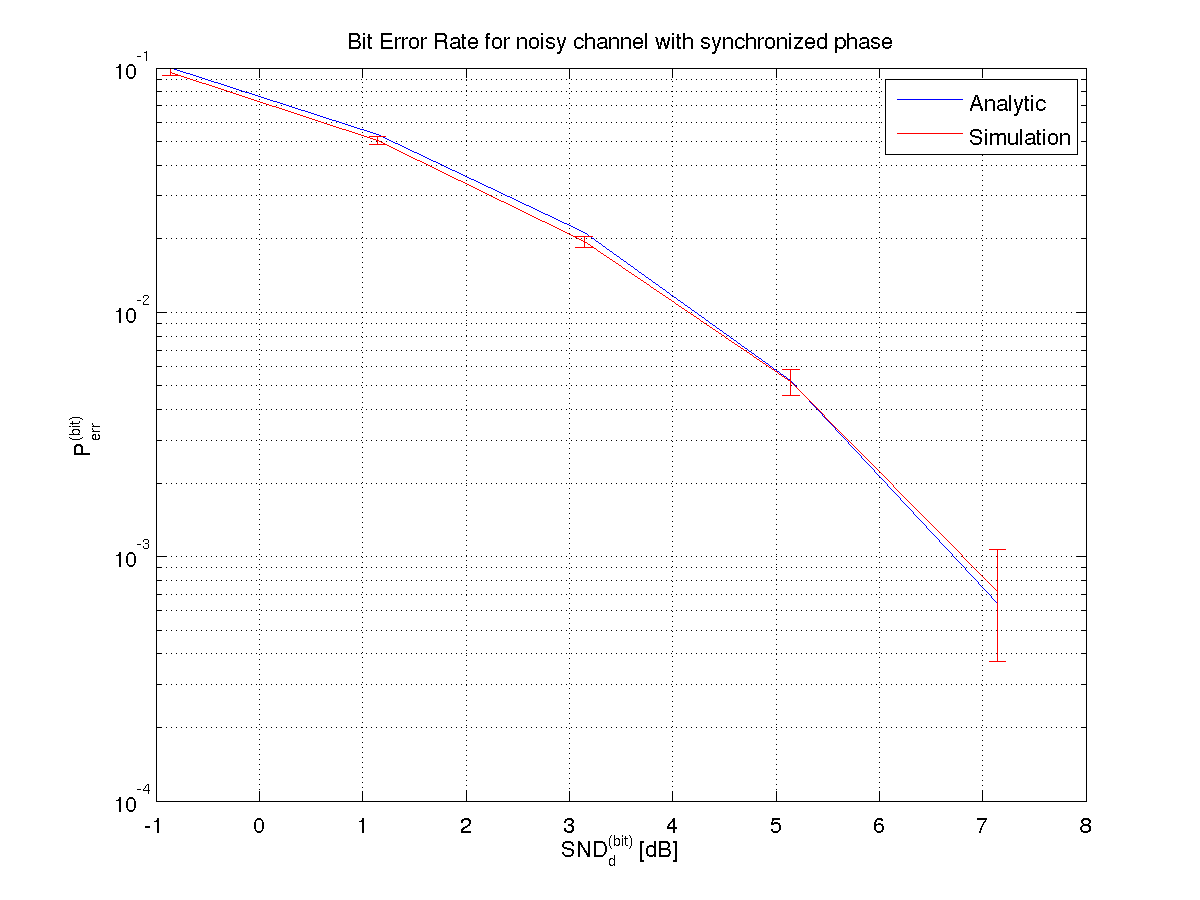
\includegraphics[height=3.5in]{BER_noise.png}
    \caption{Bit error rate of a noisy channel with ideal phase synchronization, simulated vs. analytic results}
    \label{fig:BER_noise}
  \end{figure}

  \begin{figure}[h!]
    \centering
    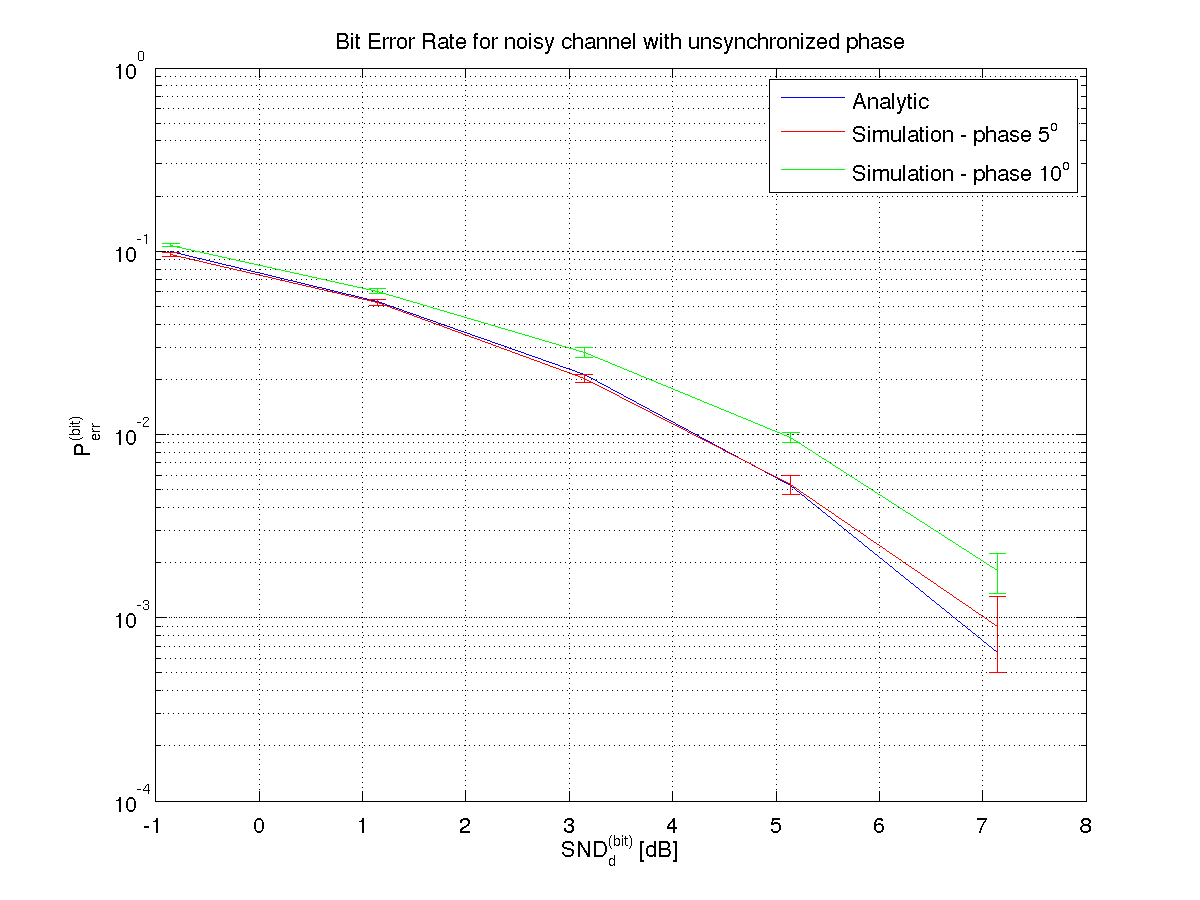
\includegraphics[height=3.5in]{BER_noise_phase.png}
    \caption{Bit error rate of a noisy channel with phase difference of $5^o$ and $10^o$, simulated vs. analytic results}
    \label{fig:BER_noise_phase}
  \end{figure}
The power penalty at $P_{err}^{(bit)} = 10^{-2}$ is calculated from the graph in Figure \ref{fig:powerpenalty} by measuring the $SNR$ difference between the analytically derived results and the results for a phase difference of $10^o$. The result shows that the power penalty is $0.83$ [dB].
  \begin{figure}[h!]
    \centering
    \includegraphics[height=3.5in]{power_penalty.png}
    \caption{Graphical calculation of the power penalty for $10^o$ phase difference at $P_{err}^{(bit)}=10^{-2}$.}
    \label{fig:powerpenalty}
  \end{figure}
Figure \ref{fig:BER_noise_constellation} demonstrates the received symbols (before decision device) for a $10^o$ constant phase and with additive noise.
  \begin{figure}[h!]
    \centering
    \includegraphics[height=3.5in]{noise_symbol_constellation.png}
    \caption{Example symbol constellation of AWGN channel with constant phase difference}
    \label{fig:BER_noise_constellation}
  \end{figure}


\clearpage
\subsection{Carrier Phase Estimation}
If the phase of the received signal varies unpredictably, symbol detection becomes a difficult problem. Knowledge of the received carrier phase allows the receiver to compensate the phase shift effect and allows for symbol detection. In this section we shall consider the case of a dispersion of $\sigma_\psi=5^o$ when $SNR_{bit} = 5$ [dB]. The phase compensation will be performed by a decision feedback loop, with a second-order transfer function. Another given parameter is $\tau_1=0.5$. The transfer function of the PLL is given by Equation 6.2.19 from \cite{Proakis}:
\begin{equation}
  \label{eq:pll_h}
  H(s) =\frac{1+\tau_2 s}{\frac{\tau_1}{K} s^2 + s \left( \frac{1}{K}+\tau_2 \right) + 1}
\end{equation}
We must choose values for $\tau_2$ and $K$. $\tau_2$ must satisfy the following properties:
\begin{itemize}
\item $\tau_2$ must be non-negative and real.
\item $\tau_2$ must be much smaller than $\tau_1$, i.e. $\tau_1 \gg \tau_2$.
\end{itemize}
We shall start by finding the equivalent PLL bandwidth, $B_{eq}$ as a function of the known parameters $\sigma_\psi^2,K_{PD},N_0$:
\begin{eqnarray*}
  \sigma_\psi^2 &=& \frac{N_0 B_{eq}}{K_{PD}^2} \\
  K_{PD} &=& \frac{A_r A_0}{2}\ \{\text{from linear model of phase detector}\}\\
  N_0 &=& \frac{P_r}{2 R_s {SNR}_{bit}} \\
  \Rightarrow B_{eq} &=& \frac{ K_{pd}^2 {\sigma}_{\psi}^2}{N_0}
\end{eqnarray*}
We recall that $B_{eq}$ is defined in terms of the transfer function, $H(s)$ (which was given in Equation \ref{eq:pll_h}):
\begin{equation*}
  B_{eq} = \frac{1}{2 \pi}\int_0^{\infty}{|H(j\omega)|^2 d\omega}
\end{equation*}
Using Equation 6.2.12 from \cite{Proakis} as the solution of the above integral, we get:
\begin{equation*}
  B_{eq}=\frac{\tau_2^2 \left( \frac{K}{\tau_1}+\frac{1}{\tau_2^2}\right) }{4 \left( \frac{1}{K}+\tau_2\right) }=\frac{\tau_2^2 {K}^2+\tau_1 K}{4 \tau_1 \tau_2 K+4 \tau_1}
\end{equation*}
Since we already know $B_{eq}$ we can treat it as a value, and write the above as a quadratic equation in $\tau_2$:
\begin{equation*}
  \tau_2^2-\frac{4 \tau_1 B_{eq}}{K}\tau_2 +\frac{\tau_1}{K}-\frac{4 \tau_1 B_{eq}} {K^2}=0
\end{equation*}
Which has solutions:
\begin{equation}
  \label{eq:tau2_k}
  \tau_{2_{a,b}}=\frac{2 \tau_1 B_{eq} \pm \sqrt{\tau_1 \left(4 \tau_1 B_{eq}^2 + 4 B_{eq} - K \right) } }{K}
\end{equation}
Recalling the restrictions on $\tau_2$ we are led to the following inequalities:
\begin{eqnarray*}
  \tau_2 \in \mathbb{R} &\Rightarrow& \tau_1 \left(4 \tau_1 B_{eq}^2 + 4 B_{eq} - K \right) \ge 0 \\
  \tau_2 \ge 0 &\Rightarrow& \left( 4 \tau_1 B_{eq}\right)^2 > \tau_1 \left(4 \tau_1 B_{eq}^2 + 4 B_{eq} - K \right)
\end{eqnarray*}
Solving for $K$ we find the condition:
\begin{equation}
  \label{eq:K_cond}
  4 B_{eq} (\tau_1 B_{eq} + 1)  > K > 4 B_{eq}
\end{equation}
Where the left inequality was changed from $\ge$ to $>$ because of the direction to find two solutions for $\tau_2$. Before substituting our values and find the allowed range of $K$, let us check how $K$ affects the damping factor:
\begin{equation*}
  \xi = \frac{\frac{1}{K}+\tau_2}{2 \sqrt{\frac{K}{\tau_1}}} 
\end{equation*}
How does $\xi$ behave when $K$ is changed? From Equation \ref{eq:tau2_k} we know that as $K$ increases, $\tau_2$ decreases. Consequently, the nominator of $\xi$ decreases and the nominator decreases. Overall, $\xi$ must also decrease with an increasing $K$. Since we have already set a constant $B_{eq}$, we can only desire a large damping factor $\xi$ - this will ensure the fastest possible convergence of the system. For this reason we pick the lower bound: $K=4 B_{eq}$. The resulting value of $\tau_2$ is simply zero, which satisfies both requirements. Now that we have found $K$ we can calculate the VCO factor $K_{VCO}$:
\begin{equation*}
  K_{VCO} = \frac{K}{K_{PD}} = \frac{8 B_{eq}}{A_r A_0}
\end{equation*}

A note about $\tau_2$: although the value of $0$ is theoretically feasible, it is safer to assume that it must be strictly greater than 0. For example, in a second-order RC circuit, a value of zero corresponds to a short (zero resistance) on the capacitor branch.

We summarize the numeric values of inputs and results of the above calculations in Table \ref{tab:k_result}.

  \begin{center}
    \begin{table}[h!]
      \centering
      \begin{tabular}[h!]{| l | l |}
      \hline 
      \bf{Name}          &  \bf{Value}  \\ \hline
      \hline
      $R_s$           &  400 [Hz] \\ \hline
      $P_r$           &  10 [W] \\ \hline
      $A_r$           &  $\sqrt{2P_r}=\sqrt{20}$ \\ \hline
      $A_0$           &  $\sqrt{2}$ \\ \hline
      $SNR_{bit}$      &  5 [dB] = $\sqrt{10}$ \\ \hline
      $\tau_1$        &  0.5 \\ \hline
      \hline
      $\sigma_{psi}$   &  $5^O = \pi / 36$  \\ \hline
      $K_{PD}$         &  $\sqrt{10}$ \\ \hline
      $B_{eq}$         &  $50 \sqrt{10}\left(\frac{\pi}{9}\right)^2 \approx 19.2656 $ \\ \hline
      $K$         &  $4 B_{eq} = 200 \sqrt{10}\left(\frac{\pi}{9}\right)^2 \approx 77.0628 $ \\ \hline
      $K_{VCO}$         &  $200 \left(\frac{\pi}{9}\right)^2 \approx 24.37$ \\ \hline
      $\tau_2$    &  $0$ \\
      \hline
      \end{tabular}
      \caption{Summary of numerical values for decision feedback loop.}
      \label{tab:k_result}
    \end{table}
  \end{center}


Figures \ref{fig:DFL} and \ref{fig:DFL_noise} show the phase error of the DFL loop without and with noise, and a constant phase difference of $5^o$. The system locks onto the phase very quickly but for reasons unsolved by the time of writing, suddenly diverges at certain points. The bits are decoded correctly.

  \begin{figure}[h!]
    \centering
    \includegraphics[height=3.5in]{phase_error_dfl.png}
    \caption{Square phase error for 5^o constant phase difference with no noise}
    \label{fig:DFL}
  \end{figure}

  \begin{figure}[h!]
    \centering
    \includegraphics[height=3.5in]{phase_error_dfl_noise.png}
    \caption{Squared Phase error for 5^o constant phase difference WITH noise}
    \label{fig:DFL_noise}
  \end{figure}

\clearpage
\bibliographystyle{IEEEtran}
\bibliography{IEEEabrv,projectbib}


\end{document}


